\documentclass[serif,mathserif]{beamer}
\usepackage{amsmath, amsfonts, epsfig, xspace}
\usepackage{algorithm,algorithmic}
\usepackage{pstricks,pst-node}
\usepackage{multimedia}
\usepackage[normal,tight,center]{subfigure}
\setlength{\subfigcapskip}{-.5em}
\usepackage{beamerthemesplit}
\usetheme{lankton-keynote}

\author[Jiong Chen]{Jiong Chen}

\title[\hspace{2em}\insertframenumber/\inserttotalframenumber]{Projective Dynamics: Fusing Constraint Projections for Fast Simulation}

\date{September 30, 2015} %leave out for today's date to be insterted

% \institute{Justice League of America}

\begin{document}

\maketitle

% \section{Introduction}  % add these to see outline in slides

\begin{frame}
  \frametitle{Position Based Dynamics}
  \begin{itemize}
    \item Force based.
      \begin{equation*}
	\text{force} \rightarrow \text{acceleration} \rightarrow \text{velocity} \rightarrow \text{position}
      \end{equation*}
    \item Position based: stable, robust, fast, visually plausible...
  \end{itemize}
  \begin{figure}[t]
      \centering
      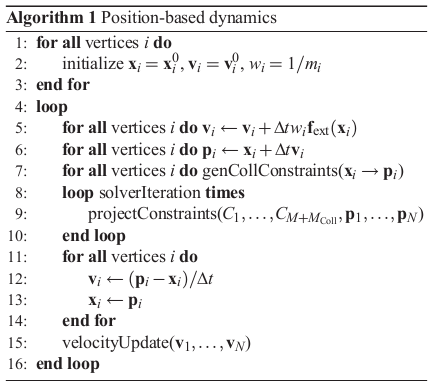
\includegraphics[scale=0.4]{pic/pbd.png}
  \end{figure}
\end{frame}

% \section{Main Body} % add these to see outline in slides

\begin{frame}
  \frametitle{Fast Simulation of Mass-Spring Systems}
  \begin{itemize}
   \item Reformulate spring potential with an auxiliary variable representing direction
    \begin{equation*}
     (\|\mathbf{p_1}-\mathbf{p_2}\|-r)^2=\underset{\|\mathbf{d}\|=r}\min~\|\mathbf{p_1}-\mathbf{p_2}-\mathbf{d}\|^2
    \end{equation*}
   with the analytic optimal solution
   \begin{equation*}
    \mathbf{d}^* = r(\mathbf{p_{12}}/\|\mathbf{p_{12}}\|)
   \end{equation*}
  The dynamics of the system then can be captured by alternating optimizing
  \begin{equation*}
   E(\mathbf{x}) = T(\mathbf{x},t)+\min_{\mathbf{d}}\frac{1}{2}\sum_{i=1}^s k_i\|\mathbf{p}_{i_1}-\mathbf{p}_{i_2}-\mathbf{d}_i\|^2+V_{other}(\mathbf{x})
  \end{equation*}

  \end{itemize}
\end{frame}

%\begin{frame}
%  \frametitle{Pictures}
%  \begin{figure}[t]
%    \centering
%    \subfigure[First Frame]{
%    \includegraphics[width=3cm]{figures/naked_leaves/00000001}}
%    \includegraphics[width=3cm]{lion.png}}
%    \subfigure[Middle Frame]{
%    \includegraphics[width=3cm]{figures/naked_leaves/00000120}}
%    \includegraphics[width=3cm]{lion.png}}
%    \subfigure[Last Frame]{
%    \includegraphics[width=3cm]{figures/naked_leaves/00000240}}
%    \includegraphics[width=3cm]{lion.png}}
%  \end{figure}
%\end{frame}

\begin{frame}
  \frametitle{Question}
  \begin{itemize}
   \item The local step to compute the optimal direction can be interpreted as projecting the springs to their 
   rest length, but unlike with PBD, spring stiffness are correctly taken into account.
   \item So, it is natural to come up with the question that how to generalize such idea to a wide variety of problems 
   such as elasticity.
  \end{itemize}
\end{frame}

% \section{Conclusion} % add these to see outline in slides

\begin{frame}
  \frametitle{Nonlinear Elasticity}
  \begin{itemize}
    \item Nonlinear elastic potentials.
      \begin{equation*}
	W(\mathbf{q}) = \Psi(\mathbf{E}(\mathbf{q}))
      \end{equation*}
    \item Decoupling distance measure and constraint manifold.
      \begin{equation*}
       W(\mathbf{p}, \mathbf{q})=d(\mathbf{p}, \mathbf{q})+\delta_{\mathbf{E}}(\mathbf{p})
      \end{equation*}
  \end{itemize}
  \begin{figure}[t]
      \centering
      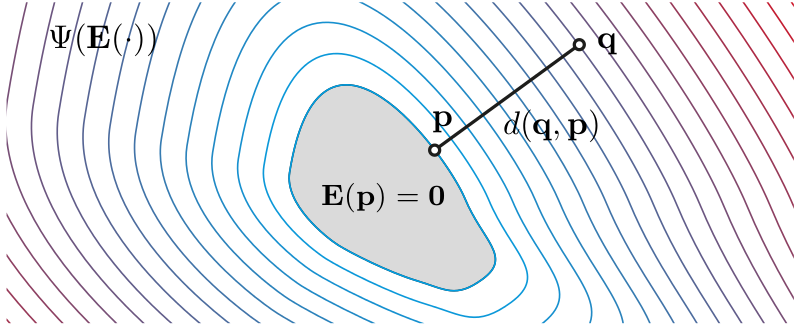
\includegraphics[scale=0.3]{pic/strain_manifold.png}
  \end{figure}
\end{frame}

\begin{frame}
  \frametitle{Nonlinear Elasticity}
  \begin{itemize}
   \item A elastic potential analogous to $\Psi(\mathbf{E}(\mathbf{q}))$
    \begin{equation*}
      \widetilde{W}(\mathbf{q})=\min_{\mathbf{p}}W(\mathbf{q}, \mathbf{p})
    \end{equation*}
    \item Quadratic distance Measures.
      \begin{equation*}
	W(\mathbf{q}, \mathbf{p})=\frac{1}{2}\|\math
      \end{equation*}
  \end{itemize}
\end{frame}

\begin{frame}
 \frametitle{Conclusion}
  \begin{itemize}
   \item handling non-linearity.
   \item discontinuous galerkin.
   \item mesh dependent.
  \end{itemize}
\end{frame}

\end{document}
